\documentclass[11pt]{article}
\usepackage[left=1in, right=1in, top=1in, bottom=1in, nohead, nofoot]{geometry}
 % see geometry.pdf on how to lay out the page. There's lots.
\geometry{letterpaper} % or letter or a5paper or ... etc
% \geometry{landscape} % rotated page geometry
\usepackage{outline}
\usepackage{amsmath}
\usepackage{graphicx}
\usepackage{epstopdf}

% See the ``Article customise'' template for come common customisations

\title{Calculation of Thermodynamic and Kinetic Properties}
\author{Wm. F. Schneider}
%\date{} % delete this line to display the current date

%%% BEGIN DOCUMENT
\begin{document}

\maketitle
%\tableofcontents
\section{Connection Between QM and Thermodynamics}
We have focused to this point on the many approaches and details of calculating
the {\em internal electronic energy} of a single molecule, that is, the energy
associated with taking infinitely separated constituent nuclei and electrons at
rest and forming a molecule:
\begin{equation}
2~\mathrm{H}^+ + 8~\mathrm{O}^{8+} + 10~\mathrm{e}^- \rightarrow
\mathrm{H_2O}~~~~~~~E^\mathrm{elec}
\end{equation}
$E^\mathrm{elec}$ is typically calculated within the Born-Oppenheimer
approximation, i.e. within the approximation that the nuclei are fixed in space
at the minimum energy configuration.  Even at 0~K, by quantum mechanics the
atoms must vibrate about this minimum, and this intrinsic vibration imparts a
{\em zero-point vibrational energy} (ZPVE) to the molecule, and the 0~K
internal energy of a molecule is thus:
\begin{equation}
  E^0=E^\mathrm{elec} + ZPVE
\end{equation}
ZPVE can be calculated reliably within the harmonic approximation, according to
\begin{equation}
  \mathrm{ZPVE}=\frac{1}{2}h\sum_{i=1}^{3n-6}\nu_i
\end{equation}
where $\nu_i$ are the harmonic vibrational frequencies, obtained from a
vibrational frequency analysis.  $E^0$ is the minimum physically meaninfful
energy of the molecule.

Energy can be deposited in a molecule in many other ways as well, e.g. as
translational and rotational kinetic energy, in excited vibrational modes, in
the interaction of a molecule with an external electric or magnetic or
gravitational field, or ....  If we assume that the energy in these various
degrees of freedom are separable, we can write:
\begin{equation}
  E_i=E^0+E^\mathrm{trans}+E^\mathrm{rot}+E^\mathrm{vib} +E^\mathrm{elec*}+E^\mathrm{ext}
\end{equation}
To fully describe microscopic energetic state of a molecule, would have to
specify all of these.

Typically, though, we are more interested in the collective properties of many
molecules at equilibrium, like the internal energy $U$ or enthalpy $H$ or Gibbs
energy $G$, under some external constraints like temperature $T$ or volu
me $V$.  These thermodynamic quantities are averages over the energy states of
an {\em ensemble} of molecules.  The way this averaging is performed is the
realm of {\em statistical thermodynamics}.

Most important for us will be the {\em canonical ensemble}, in which the free
variables are the number of molecules $N$, the total volume $V$, and the
temperature $T$.  Offer without proof, in the canonical ensemble the
probability for a molecule to be in some energy state $E_i$ above $E^0$ is
given by the Boltzmann factor,
\begin{equation}
  P(E_i) \propto e^{-E_i\beta}=e^{-E_i/k_BT},~~~~~\beta=1/k_BT
\end{equation}
Defines an exponentially decaying probability function for a state to be
occupied at some temperature.  In a sense, {\em temperature} is the property of
a system following this distribution.
\begin{figure}[h]
  \centering
  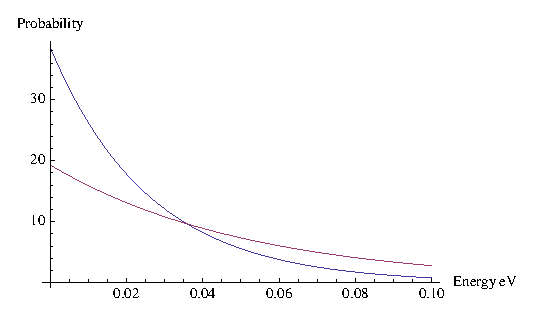
\includegraphics{boltzmann}
  \caption{Boltzmann distribution at two different temperatures}
  \label{fig:boltzmann}
\end{figure}

\subsection{Averages and partition functions}
Let's use this to calculate the internal energy $U$ of a molecule at some
temperature.  
\begin{equation}
  U(T)=\frac{\sum_iE_iP(E_i)}{\sum_iP(E_i}
\end{equation}
where the denominator ensures that the probability is normalized.
\begin{eqnarray}
  U(T) & =& \frac{\sum_iE_i e^{-E_i\beta}}{\sum_ie^{-E_i\beta}} \\
  & = & \frac{\frac{\partial}{\partial\beta}\sum_ie^{-E_i\beta}}{\sum_ie^{-E_i
      \beta}}\\
& = & -\frac{\partial \ln \sum_i e^{-E_i\beta}}{\partial \beta}
\end{eqnarray}
The sum over energy states is evidently a special quantity, called the
partition function:
\begin{equation}
  q=\sum_ie^{-E_i\beta}
\end{equation}
All thermodynamic quantities can be written in terms of the partition function!

\subsection{Harmonic oscillator example}
Harmonic oscillator is a reasonable model of a molecular vibration.  Energy
spectrum given by
\begin{equation}
  E_v=(v+1/2)h\nu,~~~~~~v=0,1,2,...
\end{equation}
Let's define the energy qunatum $h\nu=\epsilon_0$ and reset the energy scale so
that zero is at $1/2 h\nu$:
\begin{eqnarray}
  E_v & = & v\epsilon_0,~~~~~~v=0,1,2,... \\
q(T) & = &\sum_{v=0}^\infty e^{-v\epsilon_0\beta} \\
 & = & \frac{1}{1-e^{-\epsilon_0\beta}}
\end{eqnarray}
where we take advantage of the fact that the sum is a geometric series to
evaluate it in closed form. 

Plot partition function vs $T$, increasing function.

\noindent Internal energy:
\begin{eqnarray}
  U(T) &=&-\frac{\partial \ln q}{\partial \beta}\\
   & = & \frac{\epsilon_0}{e^{\epsilon_0\beta}-1}
\end{eqnarray}

\noindent Heat capacity:

\noindent Entropy

\section{Molecular Ideal Gas}
Nice example above for a simple model.  To get thermodynamics of an ideal gas,
in principle need to sum over all the types of energy states (translational,
rotational, vibrational, ...) of every molecule.  Seemingly impossible task.
One simplification is if we can write energy as sum of energies of individual
elements (molecules) of system:
    \begin{align}
      E_j&=\epsilon_j(1)+\epsilon_j(2) + ... + \epsilon_j(N) \\
      Q(N,V,T) &= \sum_j e^{-E_j\beta} \\
      &=\sum_je^{-(\epsilon_j(1)+\epsilon_j(2) + ... + \epsilon_j(N))\beta}
    \end{align}
{\em If} molecules/elements of system can be distinguished from each
        other (like atoms in a fixed lattice), expression can be factored:
      \begin{align}
        Q(N,V,T)&=\left ( \sum_j e^{-\epsilon_j(1)\beta}\right )\cdots \left ( \sum_j
          e^{-\epsilon_j(N)\beta}\right ) \\
      &= q(1)\cdots q(N) \\
      \text{Assuming all the elements are the same:}\\
      &= q^N
    \end{align}
{\em If not} distinguishable (like molecules in a liquid or gas, or
      electrons in a solid), problem is difficult, because identical
      arrangements of energy amongst elements should only be counted once.
      Approximate solution, good almost all the time:
    \begin{equation}
      Q(N,V,T)=q^N/N!
    \end{equation}
 Sidebar: ``Correct'' factoring depends on whether individual elements
      are fermions or bosons, leads to funny things like superconductivity and
      superfluidity.

This $q(V,T)$ is the {\em molecular partition function}, and is calculated by
summing over the individual energy states of a single molecule (starting at $E_0$).

Further simplified by factoring into contributions from various ($3N$) molecular
degrees of freedom:
\begin{eqnarray}
  q(V,T)&=&\left(\sum_\mathrm{trans}
    e^{-e_\mathrm{trans}\beta}\right) \left(\sum_\mathrm{rot} 
  e^{-e_\mathrm{rot}\beta}\right) \left( \sum_\mathrm{vib}
  e^{-e_\mathrm{vib}\beta} \right) \left( \sum_\mathrm{elec}
  e^{-e_\mathrm{elec}\beta}\right) \\
&=& q_\mathrm{trans}q_\mathrm{rot}q_\mathrm{vib}q_\mathrm{elec} \\
U & = & E_0 + U_\mathrm{trans}+U_\mathrm{rot}+U_\mathrm{vib}+U_\mathrm{elec} 
\end{eqnarray}
Similarly for other thermodynamic quantities, for example,
\begin{equation}
  C_v=\left(\frac{\partial U}{\partial T}\right)_V = C_{v,\mathrm{trans}}+C_{v,\mathrm{rot}}+C_{v,\mathrm{vib}}+C_{v,\mathrm{elec}}
\end{equation}
Thermodynamic quantities are sums of contributions from indvidual degrees of
freedom.

Have to somehow {\em model} these motions and have to use our quantum
mechanical results to parameterize the models.

\subsection{Translational partition function}
Need a model molecules freely translating about in a box.  How about the
{\em particle in a box}?
\begin{equation}
  E_n=\frac{n^2\pi^2\hbar^2}{2 m L^2},~~~~~n=1,2,3,...
\end{equation}
Have to construct partition function for one molecule.  For gas molecules at
normal conditions, energy spacing is tiny.  Spare the details, but find that
$q_\mathrm{trans}$ can be written in terms of a {\em thermal wavelength}
$\Lambda$:
\begin{eqnarray}
  \Lambda=\frac{h}{\sqrt{2\pi m k_B T}} \\
q_\mathrm{trans}=\frac{V^\circ}{\Lambda^3}
\end{eqnarray}
$\Lambda$ depends only a molecule mass (that's easy!) and is of the order the
box dimensions at which quantization is evident.  Typically a tiny number
(e.g. $1.7\times 10^{-11}$~m for Ar in a 1 liter volume at 298 K.
$q_\mathrm{trans}$ is, on the other hand, enormous: lots of translational
freedom.  $V^\circ$ defines the standard state volume.

Given this, can find all translational contributions to thermodynamics.
$S_\mathrm{trans}$ gives the Sackur-Tetrode equation, the absolute entropy of a
monatomic gas:


\subsection{Rotational partition function}
Model molecule as a rigidly rotating body.  Body has three orthogonal moments
of inertia $I$ determined by the molecular structure.

\subsection{Vibrational partition function}
Harmonic oscillator

\subsection{Electronic partition function}
Electronic degeneracy


{\bf do CO T-dependent thermo example}

% \item{Molecular partition function}
%   \begin{outline}
%   \item{Sum over energy states of single molecule/element of system}
%     \begin{equation}
%       q=\sum_j e^{-\epsilon_j \beta}: \mathrm{molecular\ partition\ function}
%     \end{equation}
%   \item{{\em This} can be evaluated for our QM energy models}
%   \end{outline}
%   \item{Thermodynamic quantities in terms of $q$}
%     \begin{outline}
%     \item{Internal Energy}
%       \begin{equation}
%         U(T)=-\left( \frac{\partial\ln Q}{\partial\beta} \right)_{NV}=-N\left( \frac{\partial\ln q}{\partial\beta} \right)_{V} 
%       \end{equation}
%     \item{Helmholtz Energy}
%       \begin{eqnarray}
%         A(T)=-\ln Q/\beta = -\frac{N\ln q}{\beta}~~~\mathrm{(distinguishable)} \\
%         A(T)=-\ln Q/\beta = -N\left (\ln\frac{q}{N}+1\right )/\beta~~~\mathrm{(indistinguishable)} \\
%       \end{eqnarray}
%     \end{outline}
% \end{outline}
% \item{{\bf Example: Two-level system}}
%   \begin{outline}
%   \item{$N$ distinguishable particles, each of which can have an energy of 0 or
%       $\epsilon$}
%   \item{Molecular partition function}
%     \begin{equation}
%      q = \sum_{j=1}^2 e^{-\epsilon_j\beta} = 1 + e^{-\epsilon\beta}=1 + e^{-\epsilon/k_BT}
%     \end{equation}
%   \item{Internal energy}
%     \begin{equation}
%       U(T)=-N \left ( \frac{\partial \ln(1+e^{-\epsilon\beta})}{\partial\beta}
%       \right)=\frac{N\epsilon e^{-\epsilon\beta}}{1+e^{-\epsilon\beta}}
%     \end{equation}

%   \item {Heat capacity}

%   \item {Entropy}
%   \end{outline}
% \item{{\bf Ideal monatomic gas}}
%   \begin{outline}

%   \item N identical, indistinguishable Ar atoms in a box

%   \item Particle-in-a-box energy states of one atom
%     \begin{equation}
%       \epsilon_n = \frac{n^2 \pi^2 \hbar^2}{2 m L^2}
%     \end{equation}
%   \end{outline}
% \item{{\bf Polyatomic molecular gas}}
%   \begin{outline}
%   \item Rotational energy states, rigid rotor
%   \item Vibrational energy states, harmonic oscillator
%   \end{outline}
% \item{{\bf Reaction Thermodynamics}}
% \end{outline}
\end{document}